\documentclass{article}
\usepackage[utf8]{inputenc}
\usepackage{placeins}
\usepackage{graphicx}
\usepackage{xcolor}
\graphicspath{ {./img} }

\title{Relazione Progetto di Programmazione 00819}
\author{Diego Roberto Ammirabile, \\Saad Farqad Medhat, \\Emanuele Pischetola}
\date{A.A. 2021/2022}

\begin{document}

\maketitle

\section{Scelte implementative}
% Organizzazione del progetto in 3 componenti comunicanti
% utilizzo degli eventi per comunicare
Abbiamo pensato di implementare il progetto divendendolo in tre componenti fondamentali: la vista, il modello e il controller. Questo ci è stato utile perchè i tre componenti sono abbastanza indipendenti tra di loro e ci ha permesso di lavorare in maniera asincrona.

\subsection{Modello}
Il modello è il componente che si occupa di tenere i dati del gioco. Quindi è rappresentato dalla mappa e dalle classi Room, Core, Item e le relative classi figlie.
Esso infatti viene aggiornato dal controller ogni ciclo del game loop per rispecchiare la situazione di gioco.
\\\\
\textit{Esempio: quando il giocatore preme w per muoversi verso l'alto le coordinate dell'oggetto player vengono cambiate.}

\subsection{Vista}
La vista è il componente che si occupa esclusivamente della visualizzazione grafica sul terminale, ed è rappresentato dalle classi Screen, GameMenu,\\ GameInterface, GameOptions. 
Il compito di queste classi è infatti leggere la versione più aggiornata del modello, ovvero l'oggetto di tipo Room relativo alla stanza corrente, e stampare sul terminale la corrispondente rappresentazione grafica.
\\\\
\textit{Esempio: la vista vede che le coordinate del player sono cambiate, quindi cancella il carattere del player nella posizione precedente, e poi stampa il carattere del player nelle nuove coordinate.}

\subsection{Controller}
Il controller si occupa di modificare il modello, è rappresentato da physics.h e dal main. I suoi metodi vengono invocati dalle altre classi. Questo componente deve infatti capire cosa succede nella partita, e in base a ciò creare gli eventi giusti e richiamare le funzioni necessarie.
\\\\
\textit{Esempio: controlla se i nemici nella stanza possono muoversi, se così è allora richiama il loro metodo di movimento e inserisce l'evento corrispondente al movimento di entità}

\subsection{Eventi}
Per gestire la comunicazione tra i componenti abbiamo implementato gli eventi. Ogni volta che il controller cambia qualcosa nel modello, aggiunge il relativo evento in una coda. La coda è legata alla stanza corrente, infatti è un parametro della classe Room. Quando la stampa della vista viene invocata, essa legge la coda degli eventi ed esegue la routine associata ad ogni evento che trova. 

Inoltre permettono di agire in maniera chirurgica sui caratteri dello schermo da modificare. Se, ad esempio, cambia solo la posizione del player, anziché cambiare tutto lo schermo verranno aggiornati solo due caratteri.

Gli eventi possono avere il campo data, che può essere di tipo diverso in base all'evento e contiene un'informazione utile per gestire l'evento specifico.
Gli eventi si possono trovare nel file \texttt{Events.hpp}.


\section{Divisione dei ruoli}
% Stampa a schermo e degli oggetti di gioco: piske
% Gestione della fisica: saad
% Gestione della della mappa: diego
I ruoli sono stati suddivisi in base al carico di lavoro.
La suddivisione è avvenuta nel seguente modo:
\begin{itemize}
\item \textbf{Schermo} (Emanuele Pischetola): si occupa di gestire la stampa sul terminale attraverso la librerie \texttt{curses/ncurses.h}.
\item \textbf{Entità e Oggetti} (E. Pischetola, D. Ammirabile): si tratta delle classi che descrivono tutti gli elementi rappresentabili nel gioco. Sono state realizzate tramite l'uso di ereditarietà.
\item \textbf{Fisica di gioco} (Saad Medhat): in generale si occupa di prendere in input lo stato di gioco corrente e restituire il nuovo stato di gioco, in base a ciò che è avvenuto.
\item \textbf{Mappa e Strutture dati} (Diego Ammirabile): definisce la mappa corrente e di conseguenza si occupa di memorizzare le stanze visitate e il loro contenuto
\item \textbf{Game Loop} (Diego Ammirabile): è il main file che coordina e richiama le funzioni necessarie a gestire ogni frame del gioco.
\end{itemize}

Di seguito è spiegato nello specifico chi è il responsabile di ogni file.

\subsection{Schermo}
Lo schermo è implementato nei file \texttt{Screen.hpp}, \texttt{GameInterface.hpp}, \\\texttt{GameMenu.hpp}, \texttt{GameControls.hpp}. La classe Screen è generica, mentre le altre rappresentano una specifica finestra, sono tutte create e gestite dalla classe Screen.

\subsection{Entità e Oggetti}
Le entità di gioco sono tutte figlie della classe Core, che rappresenta l'elemento di gioco più generico possibile. Le classi direttamente figlie sono Entity ovvero gli elementi "vivi", ItemOnGround cioè gli oggetti raccoglibi, e Wall i muri. 
I file sono \texttt{Core.hpp}, \texttt{ItemOnGround.hpp}, \texttt{Entity.hpp}, \texttt{Wall.hpp}, \texttt{Bullet.hpp}, \\\texttt{Player.hpp}, \texttt{Hostile.hpp}

Mentre gli oggetti che si trovano nell'inventario sono i figli della classe Item, che possono essere Consumabili come pozioni e chiavi, oppure dei potenziamenti alle statistiche come attacco e vita. Sono tutte implementate nel file \texttt{Equipment.hpp}.
C'è un file particolare, \texttt{HostileList.hpp} che contiene tutte le classi dei nemici specifici, sono tutte classe figlie di Hostile.
\\\\
Nello specifico E. Pischetola è responsabile di \texttt{Equipment.hpp}, \texttt{ItemOnGround.hpp}, \texttt{Player.hpp} e \texttt{Hostile.hpp}.
Mentre D. Ammirabile di \texttt{Wall.hpp}, \texttt{Entity.hpp}, \texttt{Bullet.hpp}.

% inserire qui schema delle classi
\begin{figure}[!ht]
    \centering
    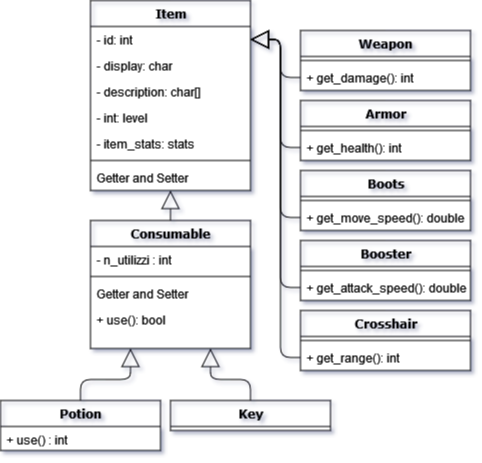
\includegraphics[width=0.7\textwidth]{UML_Prog_Programmazione_item.png}
    \caption{UML degli item}
    \label{fig:1}
\end{figure}
\FloatBarrier
\begin{figure}[!ht]
    \centering
    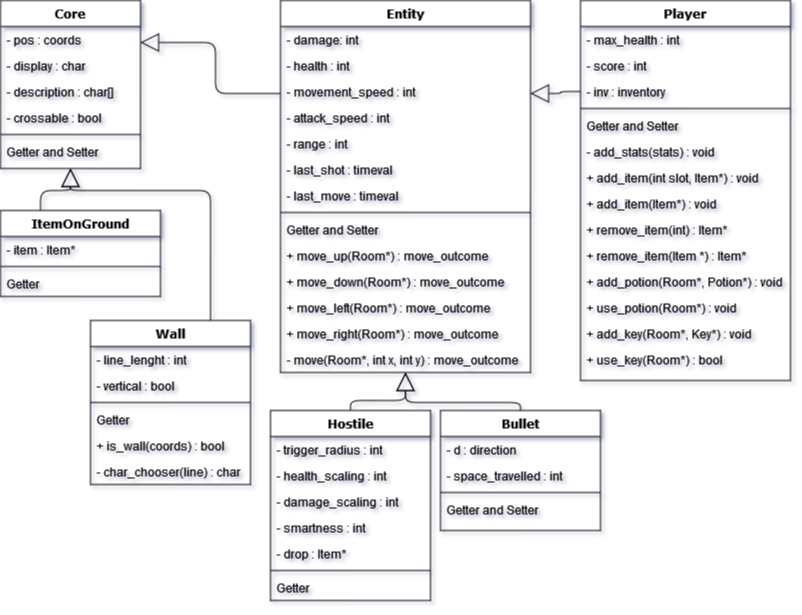
\includegraphics[width=0.95\textwidth]{UML_Prog_Programmazione.png}
    \caption{UML delle entità di gioco}
    \label{fig:2}
\end{figure}
\FloatBarrier


\subsection{Fisica di gioco}
I metodi della fisica di gioco sono raccolti nel \texttt{physics.h}. Questi metodi servono ad aggiornare lo stato di gioco, valutando ciò che è successo nell'ultimo frame e producendo le conseguenze. Agisce, ad esempio, sul movimento dei nemici, sui danni subiti, ecc.

\subsection{Mappa e Strutture Dati}
La mappa e i relativi metodi sono descritti nel file \texttt{Map.h}, ed è stata implementata tramite una struttura. Mentre la stanza è una classe implementata in \texttt{Room.hpp} e \texttt{Room\_handle.h}. Inoltre per realizzare la mappa sono state implementate due strutture dati: la lista e la coda. Sono nei file \texttt{List.hpp} e \texttt{Queue.hpp}

\subsection{Altro}
Altri file che non ho menzionato sono \texttt{constants.h} che contiene tutti i valori costanti e alcune strutture, \texttt{time\_handle.h} che ha alcune funzioni utili per calcolare il tempo in millisecondi, questi file sono di responsabilità di E. Pischetola. Mentre gli eventi, nei file \texttt{RoomEvent.hpp} e \texttt{Events.hpp}, sono di responsabilità di D. Ammirabile.

\section{Il gioco}
Di seguito si trova una descrizione di come funziona e quali sono le caratteristiche del gioco.

\subsection{Personaggio}
Il gioco permette al giocatore di controllare un personaggio identificato dalla \textbf{@}, il personaggio può sparare nelle quattro direzioni, sopra, sotto, destra, sinistra in linea retta.
Sono previste 5 statistiche: danno, vita, velocità di movimento, velocità di attacco e range. 
Inoltre il giocatore può portare con sé e trovare per terra delle pozioni e delle chiavi, le prime servono per recuperare vita e le altre per aprire delle porte bloccate.

\subsection{Oggetti}
Il giocatore può trovare 5 tipi di oggetto, ognuno aumenta una specifica statistica. In questo modo il giocatore può potenziarsi e affrontare nemici che diventano più potenti col proseguire della partita. Ogni oggetto ha un livello diverso, che cambia di quanto la statistica aumenterà una volta raccolto. Il giocatore ha 5 slot, quindi è necessario scegliere accuratamente che oggetti tenere con sé.

\subsection{Nemici}
I nemici sono di 7 tipi, ognuno con una certa peculiarità, chi fa più danno, chi ha più vita e così via. Tutti i nemici attaccano allo stesso modo del giocatore e si potenziano guadagnando vita e danno man mano che la partita va avanti.
Inoltre sono previste 3 nemici speciali, chiamati boss, che sono più forti di tutti gli altri e una volta sconfitti lasciano un oggetto. Si trovano sempre da soli.

\subsection{Mappa}
La mappa è infinita e ogni nuova stanza verrà creata nel momento in cui il giocatore passa per la porta. Le porte sono al massimo 4, ma a volte anche meno.
Le stanze essere vuote, con dei nemici, o con delle pozioni o delle chiavi. Inoltre c'è la stanza del boss che ha una sola porta e contiene un boss.

La mappa inoltre è consistente ovvero se si percorre un giro ad anello attraversando le porte si ritorna alla stanza di partenza. È possibile ritornare indietro e trovare le stanze nelle stesse condizioni in cui erano state lasciate.

\section{Strumenti utilizzati}
Per la realizzazione del progetto abbiamo utilizzato make e g++ per gestire la compilazione e l'esecuzione. Mentre per il debugging è stato usato gdb. Invece per coordinare il lavoro di gruppo git e Github.


\end{document}